\section{Coordinate Class Reference}
\label{classCoordinate}\index{Coordinate@{Coordinate}}
{\tt \#include $<$coordinate.h$>$}

Inheritance diagram for Coordinate::\begin{figure}[H]
\begin{center}
\leavevmode
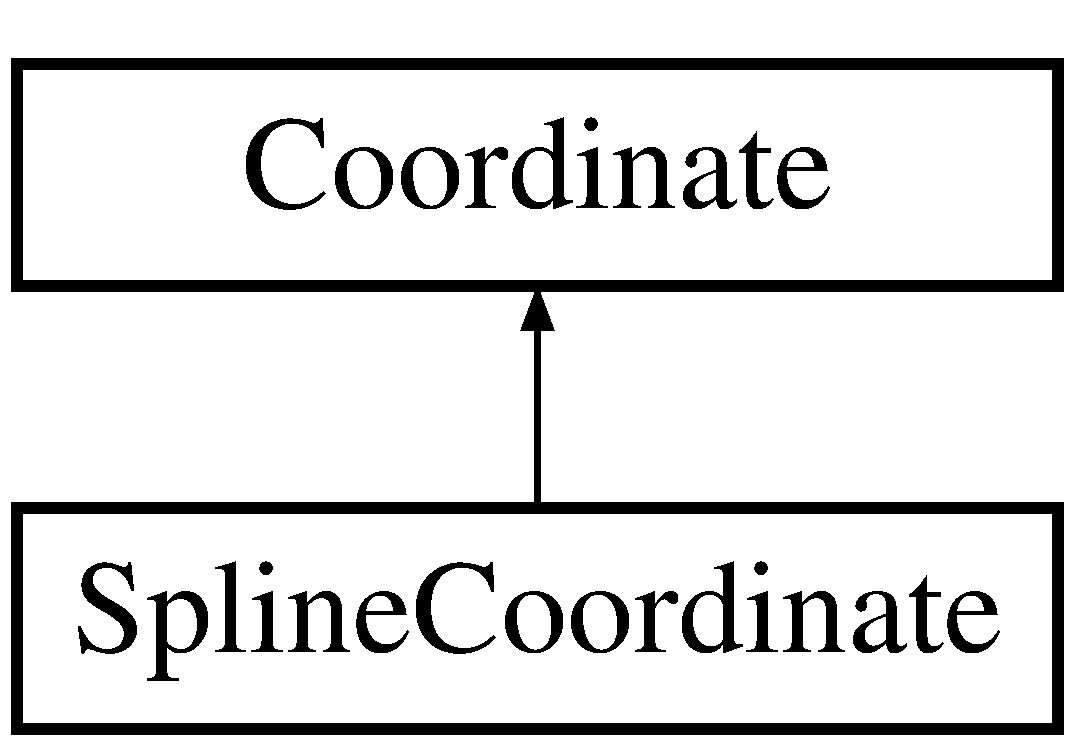
\includegraphics[height=2cm]{classCoordinate}
\end{center}
\end{figure}
\subsection*{Public Methods}
\begin{CompactItemize}
\item 
{\bf Coordinate} ()
\item 
{\bf Coordinate} (double {\bf x}, double {\bf y})
\item 
{\bf $\sim$Coordinate} ()
\item 
void {\bf set\-X} (double {\bf x})
\item 
void {\bf set\-Y} (double {\bf y})
\item 
double {\bf get\-X} ()
\item 
double {\bf get\-Y} ()
\item 
double {\bf distance} (Coordinate $\ast$c)
\item 
void {\bf write} (std::ostream \&stream) const
\end{CompactItemize}
\subsection*{Protected Attributes}
\begin{CompactItemize}
\item 
double {\bf x}
\item 
double {\bf y}
\end{CompactItemize}


\subsection{Detailed Description}
This class handles coordinates. Remember that computers use coordinate systems that are upside-down. This means that the origin of the coordinate system lays in the top-left corner, so the Y axis is upside-down... You will notice that a lot of objects use pointers to Coordinates in constructors, etc. This is because the library needs to be generic, so you can use inherited Coordinates as Coordinates too (for example {\bf Spline\-Coordinate} {\rm (p.\,\pageref{classSplineCoordinate})} instances). \begin{Desc}
\item[Author: ]\par
Anthony Liekens \end{Desc}




\subsection{Constructor \& Destructor Documentation}
\index{Coordinate@{Coordinate}!Coordinate@{Coordinate}}
\index{Coordinate@{Coordinate}!Coordinate@{Coordinate}}
\subsubsection{\setlength{\rightskip}{0pt plus 5cm}Coordinate::Coordinate ()}\label{classCoordinate_a0}


Constructor. Constructs a coordinate. \index{Coordinate@{Coordinate}!Coordinate@{Coordinate}}
\index{Coordinate@{Coordinate}!Coordinate@{Coordinate}}
\subsubsection{\setlength{\rightskip}{0pt plus 5cm}Coordinate::Coordinate (double {\em x}, double {\em y})}\label{classCoordinate_a1}


Constructor. Constructs a coordinate. \begin{Desc}
\item[Parameters: ]\par
\begin{description}
\item[{\em 
x}]Integer X-axis value of the coordinate (0 = leftmost point) \item[{\em 
y}]Integer Y-axis value of the coordinate (0 = top) \end{description}
\end{Desc}
\index{Coordinate@{Coordinate}!~Coordinate@{$\sim$Coordinate}}
\index{~Coordinate@{$\sim$Coordinate}!Coordinate@{Coordinate}}
\subsubsection{\setlength{\rightskip}{0pt plus 5cm}Coordinate::$\sim$Coordinate ()}\label{classCoordinate_a2}


Destructor. Destructs a coordinate. 

\subsection{Member Function Documentation}
\index{Coordinate@{Coordinate}!distance@{distance}}
\index{distance@{distance}!Coordinate@{Coordinate}}
\subsubsection{\setlength{\rightskip}{0pt plus 5cm}double Coordinate::distance (Coordinate $\ast$ {\em c})\hspace{0.3cm}{\tt  [inline]}}\label{classCoordinate_a7}


Returns the distance between this coordinate and another point. \begin{Desc}
\item[Parameters: ]\par
\begin{description}
\item[{\em 
c}]Coordinate of that other point \end{description}
\end{Desc}
\begin{Desc}
\item[Returns: ]\par
int \end{Desc}
\index{Coordinate@{Coordinate}!getX@{getX}}
\index{getX@{getX}!Coordinate@{Coordinate}}
\subsubsection{\setlength{\rightskip}{0pt plus 5cm}double Coordinate::get\-X ()\hspace{0.3cm}{\tt  [inline]}}\label{classCoordinate_a5}


Returns the X-axis value of the coordinate. \begin{Desc}
\item[Returns: ]\par
double \end{Desc}
\index{Coordinate@{Coordinate}!getY@{getY}}
\index{getY@{getY}!Coordinate@{Coordinate}}
\subsubsection{\setlength{\rightskip}{0pt plus 5cm}double Coordinate::get\-Y ()\hspace{0.3cm}{\tt  [inline]}}\label{classCoordinate_a6}


Returns the Y-axis value of the coordinate. \begin{Desc}
\item[Returns: ]\par
double \end{Desc}
\index{Coordinate@{Coordinate}!setX@{setX}}
\index{setX@{setX}!Coordinate@{Coordinate}}
\subsubsection{\setlength{\rightskip}{0pt plus 5cm}void Coordinate::set\-X (double {\em x})\hspace{0.3cm}{\tt  [inline]}}\label{classCoordinate_a3}


Set the X-axis value. \begin{Desc}
\item[Parameters: ]\par
\begin{description}
\item[{\em 
x}]double value \end{description}
\end{Desc}
\begin{Desc}
\item[Returns: ]\par
void \end{Desc}
\index{Coordinate@{Coordinate}!setY@{setY}}
\index{setY@{setY}!Coordinate@{Coordinate}}
\subsubsection{\setlength{\rightskip}{0pt plus 5cm}void Coordinate::set\-Y (double {\em y})\hspace{0.3cm}{\tt  [inline]}}\label{classCoordinate_a4}


Set the Y-axis value. \begin{Desc}
\item[Parameters: ]\par
\begin{description}
\item[{\em 
y}]double value \end{description}
\end{Desc}
\begin{Desc}
\item[Returns: ]\par
void \end{Desc}
\index{Coordinate@{Coordinate}!write@{write}}
\index{write@{write}!Coordinate@{Coordinate}}
\subsubsection{\setlength{\rightskip}{0pt plus 5cm}void Coordinate::write (std::ostream \& {\em stream}) const}\label{classCoordinate_a8}


Write the coordinate object to a given outstream. \begin{Desc}
\item[Parameters: ]\par
\begin{description}
\item[{\em 
stream}]output stream \end{description}
\end{Desc}
\begin{Desc}
\item[Returns: ]\par
void \end{Desc}


\subsection{Member Data Documentation}
\index{Coordinate@{Coordinate}!x@{x}}
\index{x@{x}!Coordinate@{Coordinate}}
\subsubsection{\setlength{\rightskip}{0pt plus 5cm}double Coordinate::x\hspace{0.3cm}{\tt  [protected]}}\label{classCoordinate_n0}


\index{Coordinate@{Coordinate}!y@{y}}
\index{y@{y}!Coordinate@{Coordinate}}
\subsubsection{\setlength{\rightskip}{0pt plus 5cm}double Coordinate::y\hspace{0.3cm}{\tt  [protected]}}\label{classCoordinate_n1}




The documentation for this class was generated from the following files:\begin{CompactItemize}
\item 
{\bf coordinate.h}\item 
{\bf coordinate.cpp}\end{CompactItemize}
